\begin{figure}[!htbp]
\centering
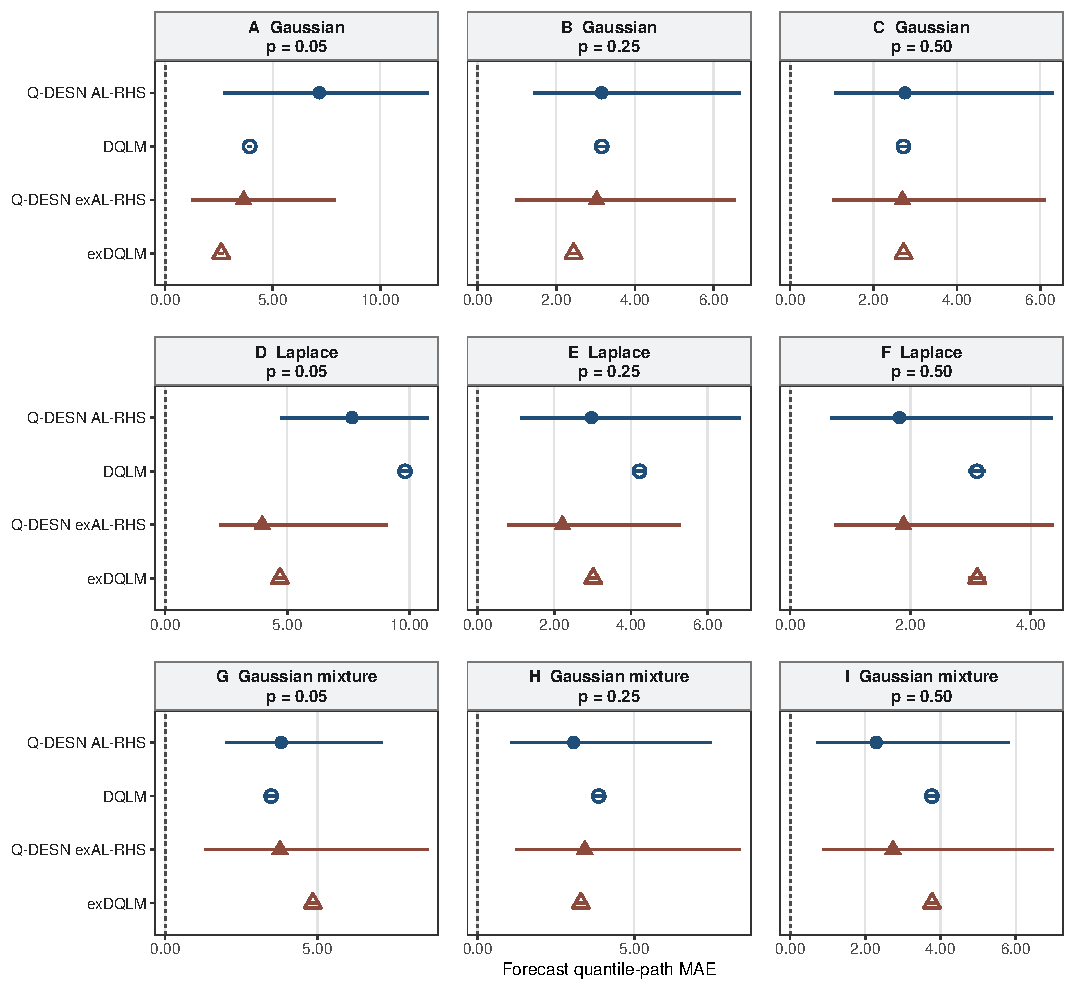
\includegraphics[width=0.98\textwidth]{figures/independent_simulation/qdesn_validation_500obs_v14_mcmc_forecast_mae_intervals.pdf}
\caption{MCMC posterior uncertainty for forecast MAE in the single-quantile
simulation. Horizontal segments show equal-tailed 95\% posterior intervals and
crosses show posterior means. Each panel has its own horizontal scale; lower is
better. The dashed line marks the exact DGP value of zero for quantile-path
error. Intervals condition on the simulated series, evaluation design, and
case-specific selected specification.}
\label{fig:simulation-500obs-mcmc-forecast-mae-intervals}
\end{figure}

\begin{figure}[!htbp]
\centering
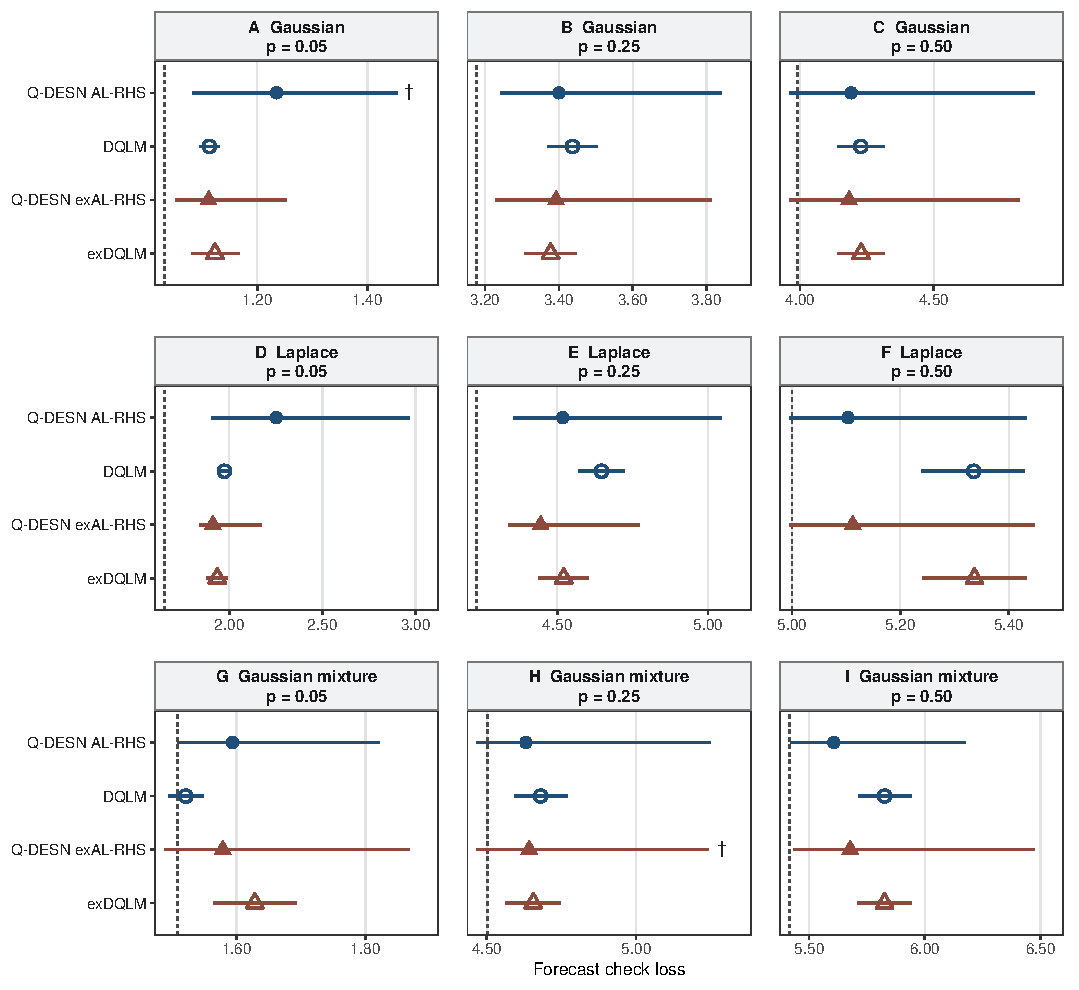
\includegraphics[width=0.98\textwidth]{figures/independent_simulation/qdesn_validation_500obs_v14_mcmc_forecast_check_loss_intervals.pdf}
\caption{MCMC posterior uncertainty for forecast check loss in the
single-quantile simulation. Horizontal segments show equal-tailed 95\%
posterior intervals and crosses show posterior means. Each panel has its own
horizontal scale; lower is better. The dashed line marks population expected
check loss at the true conditional quantile. Conditional finite-sample
intervals may cross this reference.}
\label{fig:simulation-500obs-mcmc-forecast-check-loss-intervals}
\end{figure}
